\PassOptionsToPackage{hidelinks}{hyperref}

\documentclass[stu,12pt,floatsintext]{apa7} % man doc stu jou

\usepackage[american]{babel}

\usepackage{csquotes} 
\usepackage[style=apa,sortcites=true,sorting=nyt,backend=biber]{biblatex}

\DeclareLanguageMapping{american}{american-apa}
% \addbibresource{bibliography.bib} 
\usepackage[T1]{fontenc} 
\usepackage{ctex}
\usepackage{xeCJK}
\usepackage{mathptmx} % This is the Times New Roman font, which was the norm back in my day. If you'd like to use a different font, the options are laid out here: https://www.overleaf.com/learn/latex/Font_typefaces
% Alternately, you can comment out or delete these two commands and just use the Overleaf default font. So many choices!
\setCJKmainfont{Songti SC Regular} % 设置中文主字体为 STSong,字间距增加
\setmainfont{Times New Roman} % 设置英文字体
% \renewcommand{\today}{\number\year 年 \number\month 月 \number\day 日}

%公式和列表
\usepackage{enumitem}
\usepackage{amsmath}
\usepackage{amsthm} 
\usepackage{amssymb}
\usepackage{booktabs}
\usepackage{array}     % 支持列对齐设置
\addtolength{\jot}{5pt}

%绘图用
\usepackage{subcaption}
\usepackage{graphicx}  
\usepackage{caption}
\usepackage{stfloats}
\usepackage{float}

\usepackage{pythonhighlight}

% Set up fancy header/footer
\usepackage{fancyhdr}
\pagestyle{fancy}
\fancyhead[LO,L]{2025年春学期}
\fancyhead[CO,C]{贝叶斯统计学基础}
\fancyhead[RO,R]{\number\year 年 \number\month 月 \number\day 日}
\fancyfoot[LO,L]{}
\fancyfoot[CO,C]{\thepage}
\fancyfoot[RO,R]{}
\renewcommand{\headrulewidth}{0.4pt}
\renewcommand{\footrulewidth}{0.4pt}


% Title page stuff _____________________
\title{APA Format Starter Paper, Tailored to Lab Reports But Adaptable to Other Writing Assignments} % The big, long version of the title for the title page
\shorttitle{APA Starter} % The short title for the header
\author{Your Name Here}
\duedate{April 20, 2024}
% \date{January 17, 2024} The student version doesn't use the \date command, for whatever reason
\affiliation{Your School}
\course{PSY 4321} % LaTeX gets annoyed (i.e., throws a grumble-error) if this is blank, so I put something here. However, if your instructor will mark you off for this being on the title page, you can leave this entry blank (delete the PSY 4321, but leave the command), and just make peace with the error that will happen. It won't break the document.
\professor{Dr. Professor}  % Same situation as for the course info. Some instructors want this, some absolutely don't and will take off points. So do what you gotta.

\abstract{This is the abstract for this paper, wherein the main points of the introduction, method, results, and discussion are quickly talked about. Probably in more than one sentence, though. Dare I guess, more than two? There is a page break before starting the Introduction.}

%\keywords{APA style, demonstration} % If you need to have keywords for your paper, delete the % at the start of this line


\begin{document}
\begin{titlepage}
    \centering
    \vspace*{4cm} % 调整标题的垂直位置
    \Huge
    {\heiti 贝叶斯统计学基础作业3} \\
    \vspace{1cm}
    \Large
    毛沛炫\ \ \ 3220102692 \\
    \vspace{12.3cm}
    \Large
    % \today
    \number\year 年 \number\month 月 \number\day 日
    \vfill
\end{titlepage}

\xeCJKsetup{CJKglue={\hskip 0.8pt plus 0.08\baselineskip}}



\noindent 1. {\heiti 假定对于二项分布参数 p,我们采用 beta(2,2)作为先验分布,并且进行了 10 次伯努利试验,得到了 7 次正性结果。现采用格点近似法,并使用 5 个格点,}
\begin{enumerate}[itemsep=2pt,topsep=0pt,parsep=0pt,label=(\alph*)]
    \item 计算先验分布的离散近似解(3 分)
    \item 计算后验分布的离散近似解(3 分)
    \item 计算 \(P(D)\)的近似解(3 分)
    \item 将格点数增加到 11 个,重新计算以上三个结果(4 分)
    \item 计算格点数分别为 5 和 11 时,\(P(D)\)近似解的相对误差(4 分)
\end{enumerate}


\noindent \textbf{解答:}

首先,先验概率质量分布正比于\(beta(2,2)\): 
\[
    Prior(p) \propto p^{\alpha-1}\times(1-p)^{\beta-1}  = p\times(1-p)
\]

后验分布: 
\[
    Posterior(p) \propto Likelihood(p)\times Prior(p) \propto [p^7\times(1-p)^3]\times[p\times(1-p)] = p^8\times(1-p)^4
\]

\begin{enumerate}[itemsep=2pt,topsep=0pt,parsep=0pt,label=(\alph*)]
    \item 先验分布的离散近似解
    
    令五个格点的值分别为\(\theta\) = [0.1, 0.3, 0.5, 0.7, 0.9],

    归一化之前:
    \begin{align*}
        \theta & =0.1: p = 0.1\times(1-0.1) = 0.09\\
        \theta & =0.3: p = 0.3\times(1-0.3) = 0.21\\
        \theta & =0.5: p = 0.5\times(1-0.5) = 0.25\\
        \theta & =0.7: p = 0.7\times(1-0.7) = 0.21\\
        \theta & =0.9: p = 0.9\times(1-0.9) = 0.09
    \end{align*}
    由于总和为0.85,归一化之后
    \begin{align*}
        \theta & =0.1: p = 0.1\times(1-0.1) /0.85 \approx 0.106\\
        \theta & =0.3: p = 0.3\times(1-0.3) /0.85 \approx 0.247\\
        \theta & =0.5: p = 0.5\times(1-0.5) /0.85 \approx 0.294\\
        \theta & =0.7: p = 0.7\times(1-0.7) /0.85 \approx 0.247\\
        \theta & =0.9: p = 0.9\times(1-0.9) /0.85 \approx 0.106
    \end{align*}
    上述即为先验概率分布的离散近似解
    
    \item 后验分布的离散近似解
    \begin{align*}
        \theta & =0.1: p = (0.1)^8\times(0.9)^4 \approx 6.56e-9\\
        \theta & =0.3: p = (0.3)^8\times(0.7)^4 \approx 1.58e-5\\
        \theta & =0.5: p = (0.5)^8\times(0.5)^4 \approx 2.44e-4\\
        \theta & =0.7: p = (0.7)^8\times(0.3)^4 \approx 4.67e-4\\
        \theta & =0.9: p = (0.9)^8\times(0.1)^4 \approx 4.30e-5
    \end{align*}
    归一化之后
    \begin{align*}
        p(\theta=0.1) & \approx 8.52e-06\\
        p(\theta=0.3) & \approx 0.020\\
        p(\theta=0.5) & \approx 0.317\\
        p(\theta=0.7) & \approx 0.606\\
        p(\theta=0.9) & \approx 0.056
    \end{align*}

    \item 计算 \(P(D)\)的近似解
    \begin{align*}
        P(D) & \approx \sum_{i=1}^{5}P(\theta_i)P(D|\theta_i)\\
        & = \sum_{i=1}^{5}P(\theta_i)\theta_i^7 (1-\theta_i)^3\\
        & \approx 9.058e-4
    \end{align*}

    % \begin{figure}
    %     \vspace{-1em}
    %     \centering
    %     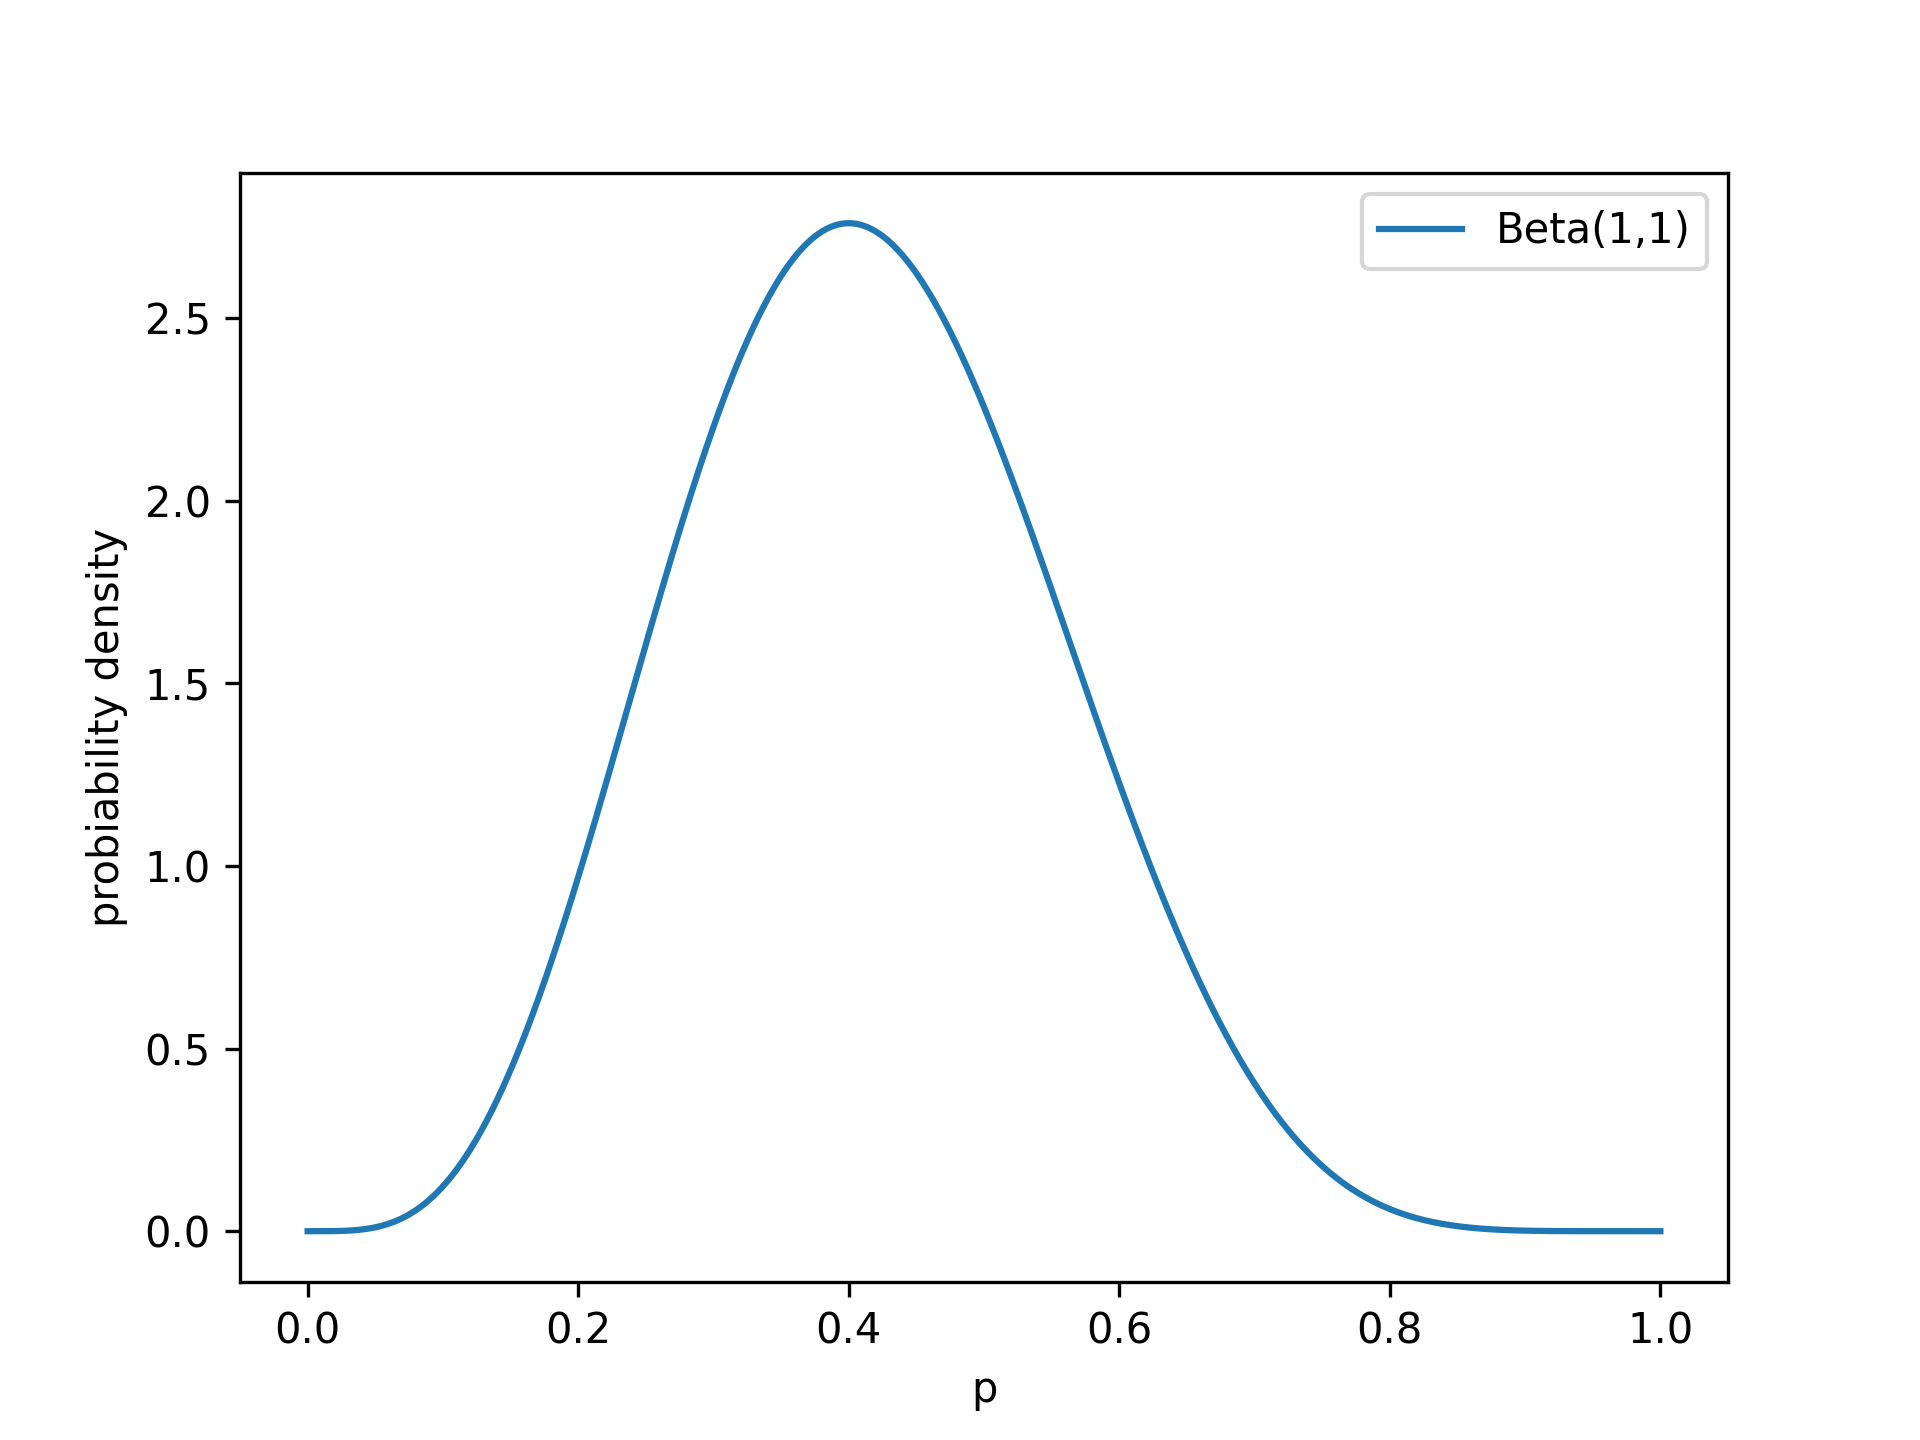
\includegraphics[width=0.6\linewidth]{figure/beta57.png} 
    %     \caption{后验贝塔分布的参数值}
    %     \label{fig:beta57}
    %     \vspace{-2em}
    % \end{figure}

    \item 将格点数增加到 11 个,重新计算以上三个结果
    
    \(\theta\)取值为:\(\theta_0 = 0.045, \theta_1 = 0.136, \theta_2 = 0.227, \theta_3 = 0.318, \theta_4 = 0.409, \theta_5 = 0.500, \theta_6 = 0.591, \theta_7 = 0.682, \theta_8 = 0.773, \theta_9 = 0.864, \theta_{10} = 0.955\)\\
    
    先验概率分布的离散近似解为(python计算给出):
    \begin{align*}
        p(\theta = 0.045) & \approx 0.024\\
        p(\theta = 0.136) & \approx 0.064\\
        p(\theta = 0.227) & \approx 0.095\\
        p(\theta = 0.318) & \approx 0.118\\
        p(\theta = 0.409) & \approx 0.131\\
        p(\theta = 0.500) & \approx 0.136\\
        p(\theta = 0.591) & \approx 0.131\\
        p(\theta = 0.682) & \approx 0.118\\
        p(\theta = 0.773) & \approx 0.095\\
        p(\theta = 0.864) & \approx 0.064\\
        p(\theta = 0.955) & \approx 0.024
    \end{align*}\\

    后验分布的离散近似解为
    \begin{align*}
        p(\theta = 0.045) & \approx 8.85e-9\\
        p(\theta = 0.136) & \approx 3.89e-5\\
        p(\theta = 0.227) & \approx 0.001\\
        p(\theta = 0.318) & \approx 0.013\\
        p(\theta = 0.409) & \approx 0.056\\
        p(\theta = 0.500) & \approx 0.143\\
        p(\theta = 0.591) & \approx 0.244\\
        p(\theta = 0.682) & \approx 0.280\\
        p(\theta = 0.773) & \approx 0.198\\
        p(\theta = 0.864) & \approx 0.063\\
        p(\theta = 0.955) & \approx 0.002
    \end{align*}

    \(P(D)\)的近似解为\(P(D) \approx 9.285e-4\)

    \item 计算格点数分别为 5 和 11 时,P(D)近似解的相对误差
    
    \(P(D)\)的精确值为
    \begin{align*}
        P(D) & = \int_0^1 p(\theta)p(D|\theta)d\theta\\
        & = \int_0^1 \frac{\Gamma(4)}{\Gamma(2)\Gamma(2)} \theta(1-\theta) \theta^7 (1-\theta)^3 d\theta\\
        & = \int_0^1 6 \theta^8 (1-\theta)^4 d\theta\\
        & = \frac{2}{2145}
    \end{align*}\\

    所以5个格点的相对误差是
    \[
    \frac{\left|P_{N=5}(D) - \frac{2}{2145}\right|}{\frac{2}{2145}} = 2.587\%
    \]

    所以11个格点的相对误差是
    \[
    \frac{\left|P_{N=11}(D) - \frac{2}{2145}\right|}{\frac{2}{2145}} = 0.422\%
    \]

\end{enumerate}

\noindent 2. {\heiti 使用 JASP 中名为 Heart Rate 的数据集,进行贝叶斯方差分析,考察各个因素是否存在主效应,以及是否存在交互效应。根据贝叶斯因子选取和报告最优模型,并且报告针对各种效应的贝叶斯因子和相应的统计推断。(6 分)}

\noindent \textbf{解答:}


\begin{table}[H]
    \centering
    \caption{模型比较}
    \label{tab:modelComparison}
    \resizebox{\linewidth}{!}{
        \begin{tabular}{lrrrrr}
            \toprule
            Models & P(M) & P(M|data) & BF$_{M}$ & BF$_{10}$ & error \%  \\
            \cmidrule[0.4pt]{1-6}
            Gender + Group + Gender * Group & $0.200$ & $0.794$ & $15.388$ & $1.000$ & \\
            Gender + Group & $0.200$ & $0.206$ & $1.040$ & $0.260$ & $2.560$  \\
            Group & $0.200$ & $6.696\times10^{-36}$ & $2.678\times10^{-35}$ & $8.436\times10^{-36}$ & $2.320$  \\
            Gender & $0.200$ & $1.809\times10^{-107}$ & $7.234\times10^{-107}$ & $2.279\times10^{-107}$ & $2.320$  \\
            Null model & $0.200$ & $2.296\times10^{-126}$ & $9.185\times10^{-126}$ & $2.893\times10^{-126}$ & $2.320$  \\
            \bottomrule
        \end{tabular}
    }
\end{table}

\indent 全因子模型的贝叶斯因子\(BF_{10}\)远大于100(见Table\ref{tab:modelComparison}),说明数据有极强的证据支持全因子模型而非空模型。且和其他模型相比,全因子模型的\(BF_{M\bar{M}}\)=15.388,且其他模型的\(BF_{M\bar{M}}\)均小于3,说明数据有较强的证据支撑全因子模型而非其他模型。

\begin{table}[H]
	\centering
	\caption{效应分析}
	\label{tab:analysisOfEffects-HeartRate}
	\resizebox{\linewidth}{!}{
        \begin{tabular}{lrrrrr}
			\toprule
			Effects & P(incl) & P(excl) & P(incl|data) & P(excl|data) & BF$_{incl}$  \\
			\cmidrule[0.4pt]{1-6}
			Gender & $0.400$ & $0.400$ & $0.206$ & $6.696\times10^{-36}$ & $3.081\times10^{+34}$  \\
			Group & $0.400$ & $0.400$ & $0.206$ & $1.809\times10^{-107}$ & $1.141\times10^{+106}$  \\
			Gender * Group & $0.200$ & $0.200$ & $0.794$ & $0.206$ & $3.847$  \\
			\bottomrule
			% \addlinespace[1ex]
			% \multicolumn{6}{p{0.5\linewidth}}{\textit{Note.} Compares models that contain the effect to equivalent models stripped of the effect. Higher-order interactions are excluded. Analysis suggested by Sebastiaan Mathôt.} \\
		\end{tabular}
        }
\end{table}

\vspace{1em}
\indent 选择JASP的默认参数,并和最佳模型进行比较。效应分析中,Gender和Group的\(BF_{incl}\)都远大于100(见Table\ref{tab:analysisOfEffects-HeartRate}),根据Wagenmakers, Love等人提出的分类标准,说明数据有极强的证据支持了不同Gender的人在心率上具有差异,不同Group的人在心率上具有差异,Gender和Group的主效应显著。而Group*Gender的贝叶斯因子为\(BF_{incl}\) = 3.847, 说明在(假定有效应的)备择假设下出现当前数据的可能性是在(假定没有效应的)零假设下可能性的3.847倍。根据分类标准, 这是中等程度的证据支持了备择假设, Gender和Group之间存在交互作用。\\

\vspace{1em}
\noindent 3. {\heiti  使用 JASP 中名为 Auction 的数据集,进行贝叶斯回归分析。具体要求如下:以 Age 和 Bidders 为自变量,Price 为因变量,考虑所
有可能模型(包括含交互项的模型,且各模型的先验概率应当相等),并根据贝叶斯因子选取和报告最优模型,以及各回归系数的后验 90\%可信区间}


\vspace{1em}
使用jasp默认参数(各模型的先验概率相等。最优模型(见Table\ref{tab:modelComparison-Price})为包含交互项的模型(Age + Bidders + Age × Bidders)。贝叶斯因子 \(BF_M\) = 38784.660,表明该模型比其他模型有极强的证据支持(BF > 100);R\(^2\) = 0.954,说明模型对数据的解释力极高。
Age + Bidders 模型的 \(BF_{10}\) = 1.031×10\(^2\),和最优模型相比,数据对该模型的支持证据极弱。\\

\begin{table}[H]
	\centering
	\caption{模型比较}
	\label{tab:modelComparison-Price}
	\resizebox{\linewidth}{!}{
		\begin{tabular}{lrrrrr}
			\toprule
			Models & P(M) & P(M|data) & BF$_{M}$ & BF$_{10}$ & R$^{2}$  \\
			\cmidrule[0.4pt]{1-6}
			Age + Bidders + Age * Bidders & $0.200$ & $1.000$ & $38784.660$ & $1.000$ & $0.954$  \\
			Age + Bidders & $0.200$ & $1.031\times10^{-4}$ & $4.125\times10^{-4}$ & $1.031\times10^{-4}$ & $0.893$  \\
			Age & $0.200$ & $1.105\times10^{-12}$ & $4.420\times10^{-12}$ & $1.105\times10^{-12}$ & $0.533$  \\
			Bidders & $0.200$ & $4.528\times10^{-16}$ & $1.811\times10^{-15}$ & $4.529\times10^{-16}$ & $0.156$  \\
			Null model & $0.200$ & $1.782\times10^{-16}$ & $7.127\times10^{-16}$ & $1.782\times10^{-16}$ & $0.000$  \\
			\bottomrule
		\end{tabular}
	}
\end{table}

%----- Requires booktabs package -----%

\begin{table}[H]
	\centering
	\caption{根据后验分布的系数估计}
	\label{tab:posteriorSummariesOfCoefficients}
	\resizebox{\linewidth}{!}{
		\begin{tabular}{lrrrrrrrrr}
			\toprule
			\multicolumn{1}{c}{} & \multicolumn{1}{c}{} & \multicolumn{1}{c}{} & \multicolumn{1}{c}{} & \multicolumn{1}{c}{} & \multicolumn{1}{c}{} & \multicolumn{1}{c}{} & \multicolumn{1}{c}{} & \multicolumn{2}{c}{90\% Credible Interval} \\
			\cline{9-10}
			Coefficient & P(incl) & P(excl) & P(incl|data) & P(excl|data) & BF$_{inclusion}$ & Mean & SD & Lower & Upper  \\
			\cmidrule[0.4pt]{1-10}
			Intercept & $1.000$ & $0.000$ & $1.000$ & $0.000$ & $1.000$ & $1327.156$ & $15.621$ & $1298.693$ & $1352.459$  \\
			Age & $0.400$ & $0.400$ & $1.031\times10^{-4}$ & $6.310\times10^{-16}$ & $1.634\times10^{+11}$ & $0.867$ & $2.012$ & $-2.799$ & $4.125$  \\
			Bidders & $0.400$ & $0.400$ & $1.031\times10^{-4}$ & $1.105\times10^{-12}$ & $9.330\times10^{+7}$ & $-92.697$ & $29.594$ & $-146.621$ & $-44.762$  \\
			Age * Bidders & $0.200$ & $0.200$ & $1.000$ & $1.031\times10^{-4}$ & $9696.165$ & $1.288$ & $0.210$ & $0.905$ & $1.628$  \\
			\bottomrule
		\end{tabular}
	}
\end{table}

模型中各个因子的回归系数和后验90\%可信区间(见Table\ref{tab:posteriorSummariesOfCoefficients}):\\
交互项 Age × Bidders:\\
回归系数为1.288 ,90\% 可信区间为 (0.905, 1.628)。\\
Bidders:\\
回归系数为-92.697  ,90\% 可信区间为 (-146.62, -44.76)\\
Age:\\
回归系数为0.867  ,90\% 可信区间为 (-2.799, 4.125)\\
截距:\\
回归系数为1327.156 ,90\% 可信区间为 (1298.69, 1352.46)\\


\vspace{1em}
\noindent 4. {\heiti 使用 JASP 中名为 Emily Rosa 的数据集,进行贝叶斯二项检验。具体要求如下:以 correct 比例为 0.46,incorrect 比例为 0.54作为零假设,以 correct 比例满足 beta(2.3,2.7)为被择假设的先验分布,进行统计检验,并报告相应的贝叶斯因子,correct 比例的后验 95\%可信区间,以及统计推断结果}


\begin{table}[h]
	\centering
	\caption{贝叶斯二项分布检验}
	\label{tab:bayesianBinomialTest}
	{
		\begin{tabular}{ l p{0.15\linewidth}<{\raggedright}p{0.15\linewidth}<{\raggedright}p{0.15\linewidth}<{\raggedright}p{0.15\linewidth}<{\raggedright} p{0.15\linewidth}<{\raggedright}}
			\toprule
			 & Level & Counts & Total & Proportion & BF$_{1}$$_{0}$  \\
			\cmidrule[0.4pt]{1-6}
			Outcome & Correct & $70$ & $150$ & $0.467$ & $0.173$  \\
			$ $ & Incorrect & $80$ & $150$ & $0.533$ & $0.817$  \\
			\bottomrule
			\addlinespace[1ex]
			\multicolumn{6}{p{0.9\linewidth}}{\textit{Note.} Proportions tested against value: 0.46. The shape of the prior distribution under the alternative hypothesis is specified by Beta(2.3, 2.7).} \\
		\end{tabular}
	}
\end{table}

设置 correct 比例为 0.46,incorrect 比例为 0.54作为零假设,以 correct 比例满足 beta(2.3,2.7)为被择假设的先验分布,检验方向为\(\neq\)Test value,其他参数按照JASP默认值,进行分析,结果见Table\ref{tab:bayesianBinomialTest}和Figure\ref{fig:BinomialTestPlot}

\begin{figure}[H]
    \centering
    \begin{minipage}{0.48\textwidth}
        \centering
        \subcaption{}
        \vspace{-0.5em}
        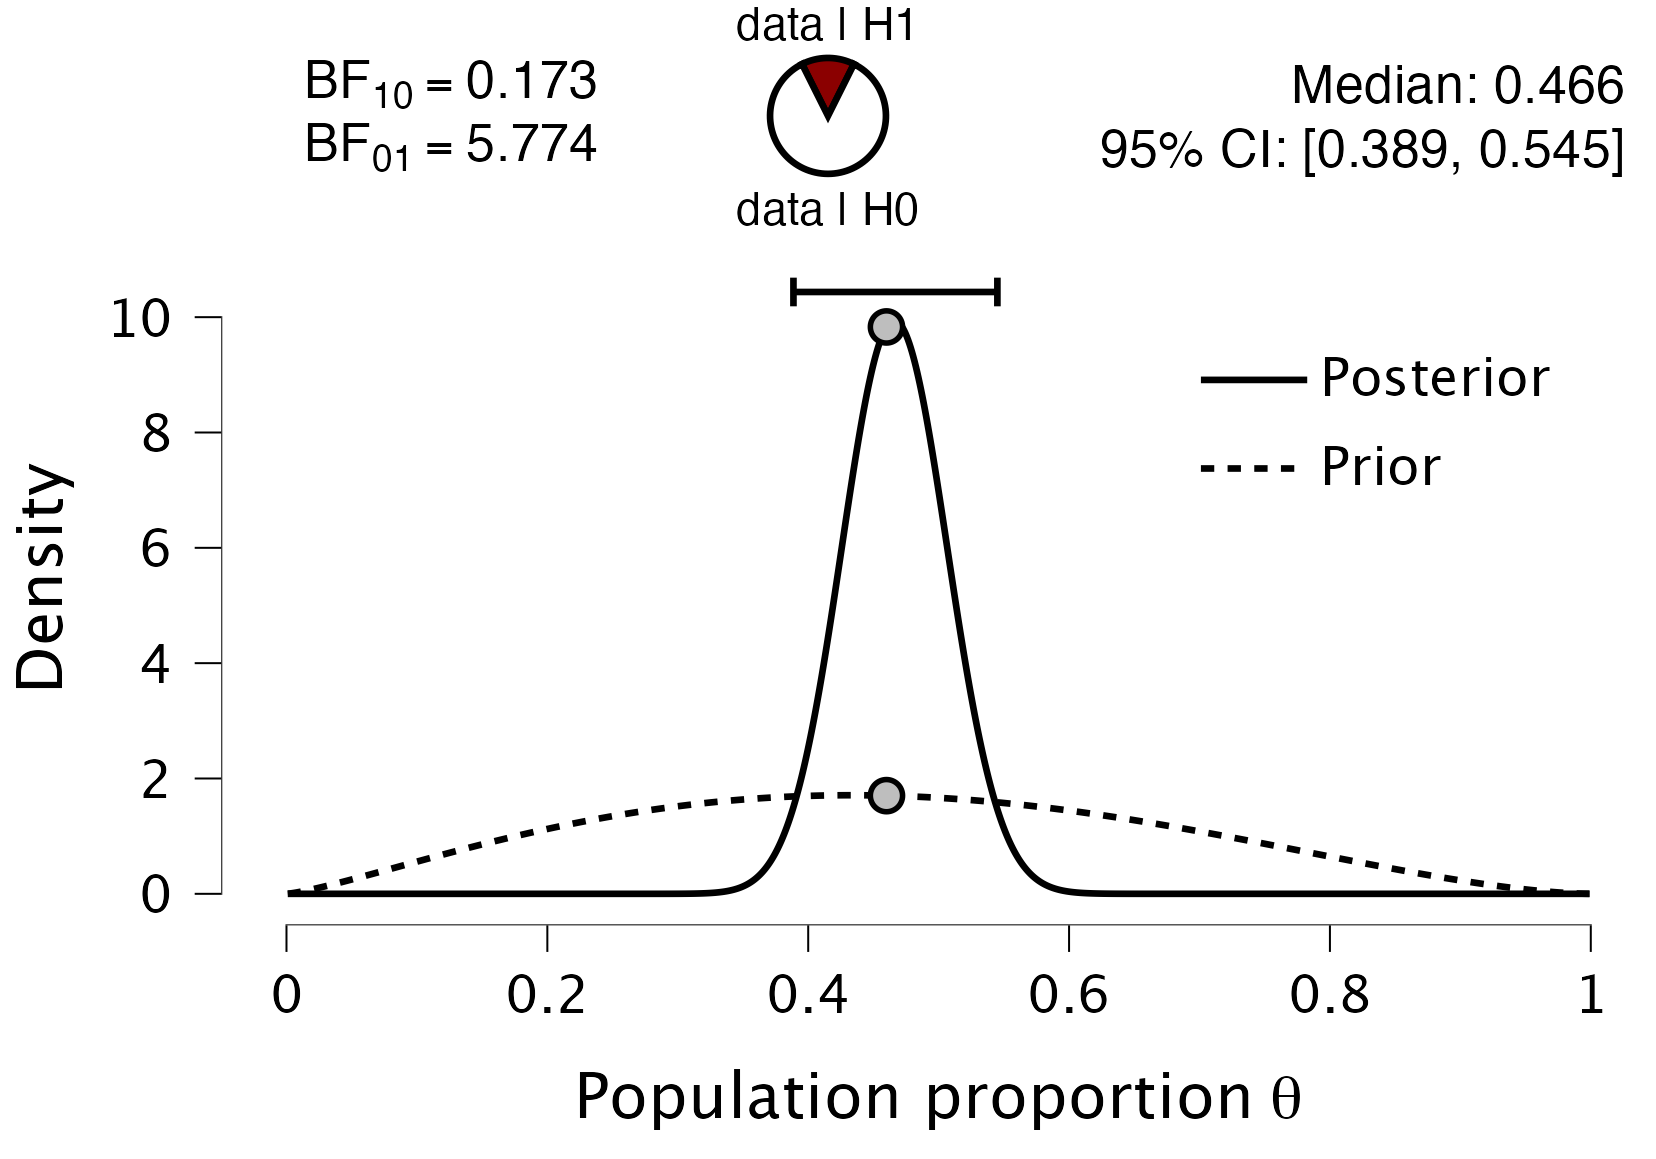
\includegraphics[width=\textwidth]{figure/correct.png}
        \label{fig:correct}
    \end{minipage}
    \begin{minipage}{0.48\textwidth}
        \centering
        \subcaption{}
        \vspace{-0.5em}
        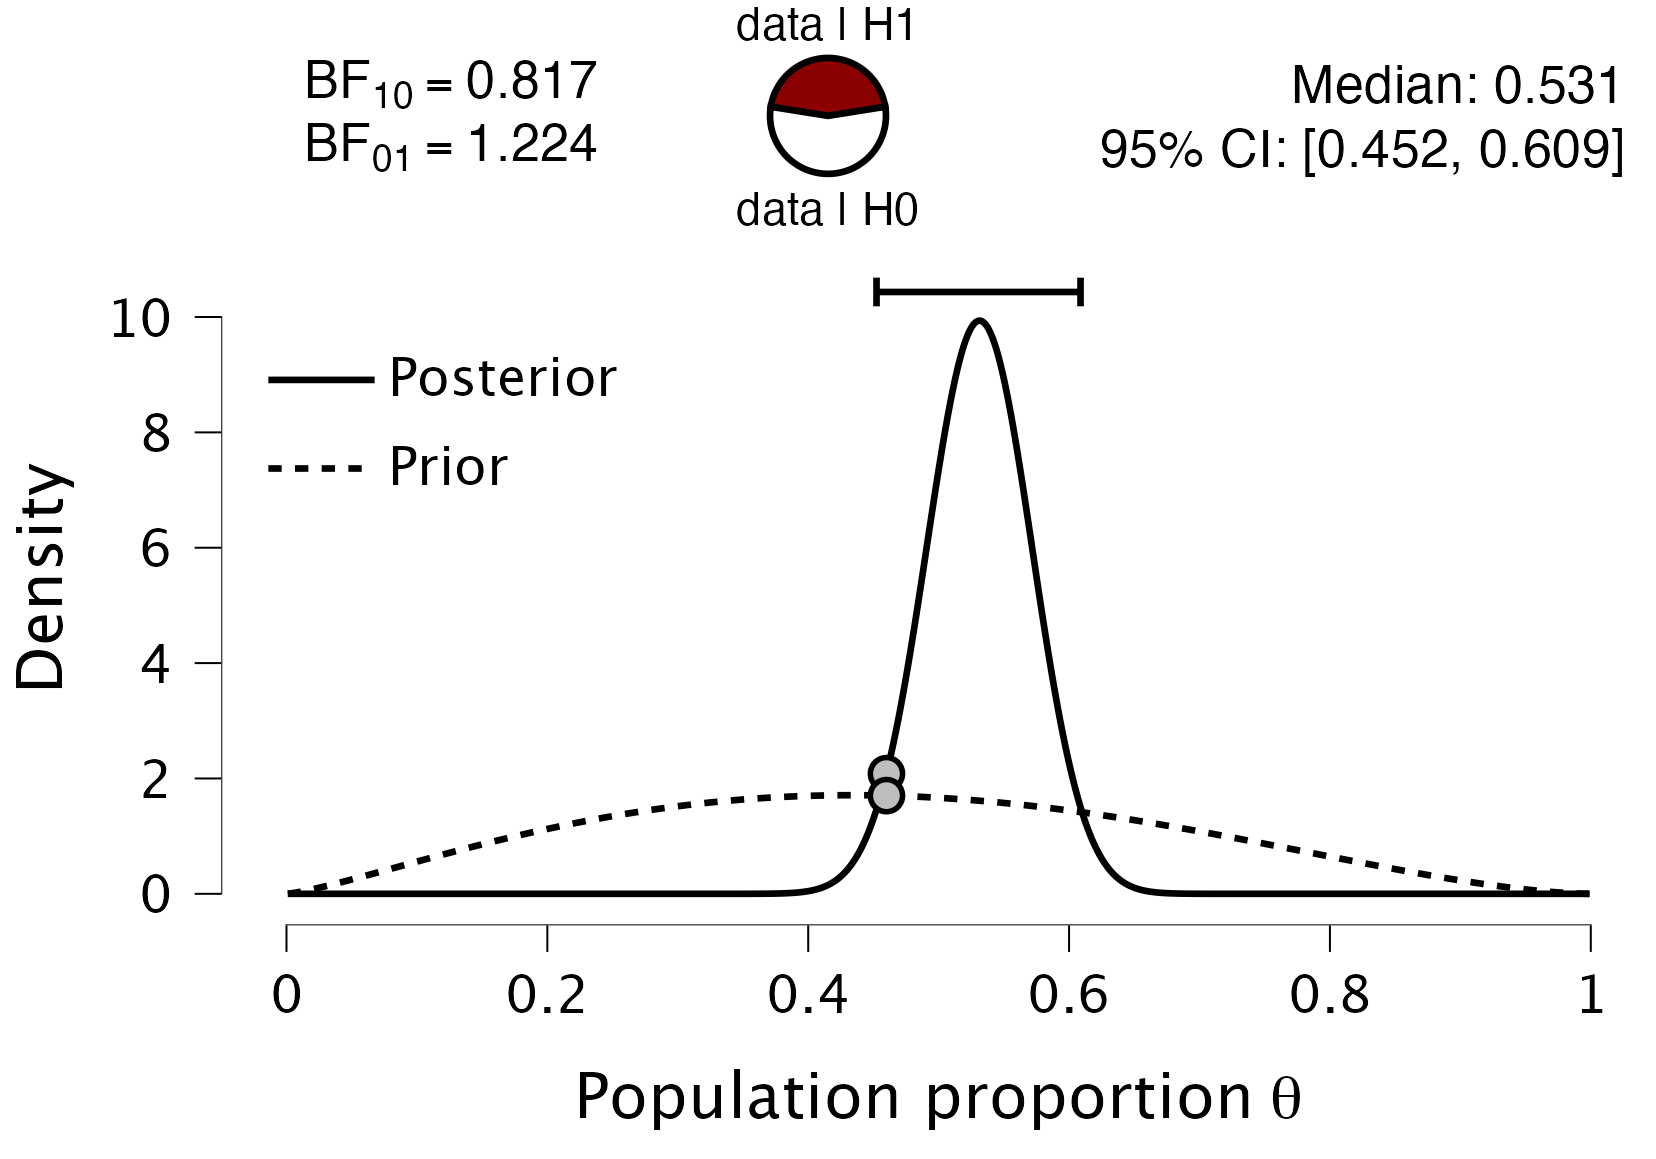
\includegraphics[width=\textwidth]{figure/incorrect.png}
        \label{fig:incorrect}
    \end{minipage}
    \captionsetup{labelsep=period}
    \caption{\rm (a)\ correct比例的先验分布和后验分布;(b)\ incorrect比例的先验和后验分布}
    \label{fig:BinomialTestPlot}
\end{figure}

根据分析结果,贝叶斯因子 \(BF_{10}\) = 0.173,表示当前数据支持零假设(correct 比例为 0.46)的证据比支持被择假设的证据强约 5.774 倍。这表明有中等程度的证据支持零假设,即有中等强度的证据支持correct 比例为 0.46。correct 比例的后验 95\%可信区间为(0.389, 0.545)


\end{document}
